The implementation of the breast cancer detection system was conducted in two parts. The first part corresponds to a common pipeline developed in group, and the second part to individual implementations using the common pipeline as a baseline. The distribution of work during the implementation of the common pipeline can be found in Appendix~\ref{ch:appendix-team-meeting-summaries}.

%%%%%%%%%%%%%%%%%%%%%%%%%%%%%%%%%%%%%%%%%%%%%
%%%%%%%%%%%%%%%%%%%%%%%%%%%%%%%%%%%%%%%%%%%%%
%%%%%%%%%%%%%%%%%%%%%%%%%%%%%%%%%%%%%%%%%%%%%

\section{Code Design}

The code is designed by splitting essential code into functions spread across multiple python modules, which are all organised into different directories based on what task they accomplish.

The entry point is in the ``main.py'' module, which parses command line arguments used to execute different parts (e.g. which dataset to use). It contains the main flow of execution with calls to functions for processing the data, creating the CNN models and evaluating the results.\\

Functions linked to data pre-processing, such as retrieving image paths and labels, processing images, encoding labels, loading the data into memory and transforming images for data augmentation, are all located in the \textit{data\_operations} directory. One-time scripts for parsing the images' paths and labels for each dataset are in the \textit{dataset\_processing\_scripts} directory.\\

All CNN-related code, such as creating the model, compiling it, fitting, making predictions or evaluating it is placed in a custom \textit{CNN\_Model} class, which can be found in the \textit{cnn\_models.py} module. Separate models, such as VGG or InceptionV3, are individually placed the \textit{cnn\_models} directory.\\

Functions handling result visualisations in the form of plots and CSV reports are all situated in the \textit{data\_visualisation} directory.\\

General functions for printing information in the terminal and common operations are all located in the \textit{utils.py} module, while global command line arguments used throughout the code are all stored in the \textit{config.py} module.


%%%%%%%%%%%%%%%%%%%%%%%%%%%%%%%%%%%%%%%%%%%%%
%%%%%%%%%%%%%%%%%%%%%%%%%%%%%%%%%%%%%%%%%%%%%
%%%%%%%%%%%%%%%%%%%%%%%%%%%%%%%%%%%%%%%%%%%%%

\section{Common Deep Learning Pipeline}

A detailed flowchart of the deep learning pipeline implemented can be found in  Figure~\ref{fig:implementation-detailed-flowchart}.

\begin{figure}[ht]
\centerline{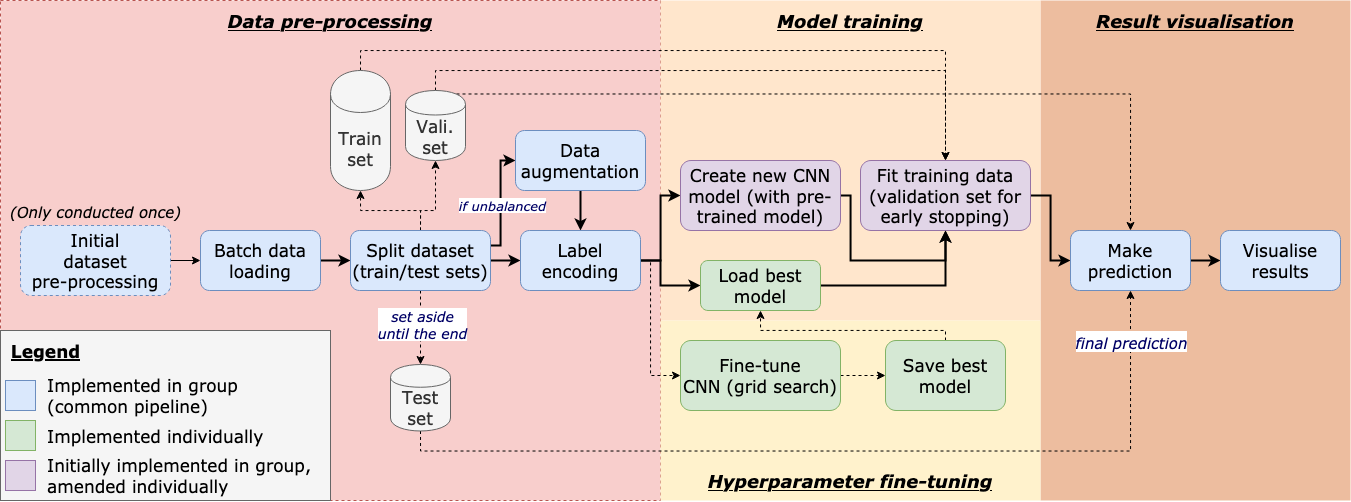
\includegraphics[width=1.25\textwidth]{Dissertation/figures/implementation/detailed flowchart.png}}
\caption{\label{fig:implementation-detailed-flowchart}Flowchart. Created using draw.io.}
\end{figure}

%%%%%%%%%%%%%%%%%%%%%%%%%%%%%%%%%%%%%%%%%%%%%

\subsection{Data pre-processing}

\subsubsection{Initial dataset processing}

Two Python scripts written to initially parse CSV files mapping image paths and their labels in order to reorganise the images in labelled folders for classification.\\

File formats: PGM and DICOM files converted to arrays to be readable by the CNNs as input.\\

%%%%%%%%%%%

\subsubsection{Data loading}

Processed CSV files containing image paths are parsed to generate a list of all images and a list of all labels.\\

Tensorflow cache and batch functions used to load the CBIS-DDSM dataset.\\

No optimisations used for the smaller mini-MIAS dataset (just the Keras \textit{img\_to\_array} and \textit{load\_img} functions).\\

%%%%%%%%%%%

\subsubsection{Image processing}

For mini-MIAS, images are loaded, resized to a target size (1024x1024 or 224x224 pixels), converted to an array format and normalised.\\

Images resized on import to match the input size of the pre-trained model. For instance, VGG19 takes 224x224px images.\\

Normalising images to fit in [0-1] float range rather than [0-255] integer range.\\

Scikit-Learn's \textit{LabelEncoder} class is used to one-hot encode labels and Keras' \textit{to\_categorical}  function is used to convert to a binary class matrix usable by the CNN models.\\

A 60/20/20\% shuffled stratified split (maintain class balance across split sets) is used for the mini-MIAS dataset. A default 80/20\% train test split is already done for CBIS-DDSM dataset, and the training set is further split into 75/25\% for a total 60/20/20\% split.\\

Class weights are calculated automatically using sklearn's \textit{class\_weight}.\\

For the mini-MIAS dataset, images are cropped around a ROI (Region of Interest) sized 224x224 pixels if there is one, otherwise around a 224x224 region around the centre of the image.\\

Data augmentation for the mini-MIAS  dataset images to balance the class distribution. Rotations, noise, shears and rotation flips are randomly added to existing images to create new images and to balance classes. These are then shuffled to ensure that newly generated images are not grouped together.

%%%%%%%%%%%%%%%%%%%%%%%%%%%%%%%%%%%%%%%%%%%%%

\subsection{Model training}

A VGG19 pre-trained model (using ImageNet weights) is used through the Keras API. The fully connected layers are replaced with new fully connected layers to accommodate the breast cancer detection classes (benign and malignant for CBIS-DDSM, and normal as well for mini-MIAS).\\

Training is conducted in two phases:
\begin{itemize}
    \item During the first phase, the VGG19 layers are frozen (weights are not updated during training) and only the fully connected layers are being updated. This is done by setting the \textit{trainable} attribute for the layers in question to False.
    \item Once the first training phase is stopped (using early stopping when the validation loss does not improve after 8 epochs), all the layers are unfrozen and training is resumed at a lower learning rate for the VGG19 models to adapt to the mammograms images.
\end{itemize}

Additional convolution and spooling layers are added before the pre-trained model to accommodate larger images. These are slowly reduced in size as they go through the spooling layers, allowing lower-level features to be learned before passing through the VGG19 model.\\

Once the CNN model is finished training model is saved in HDF5 format in order to save the model's architecture, the layers' hyperparameters, all the connection weights and biases that were learned during training \citep{Geron2019} and the optimiser used.

%%%%%%%%%%%%%%%%%%%%%%%%%%%%%%%%%%%%%%%%%%%%%

\subsection{Results visualisation}

Scikit-Learn's \textit{classification\_report} and \textit{accuracy\_score} functions used to get numerical result metrics.\\

Matplotlib used to plot the ROC curve and seaborn for the confusion matrices.

%%%%%%%%%%%%%%%%%%%%%%%%%%%%%%%%%%%%%%%%%%%%%

\subsection{General}

Python's \textit{argparse} is used to implemenent the CLI application, accepting different arguments such as the dataset to use, the CNN model to use, whether to train or test the model, etc. (see Appendix~\ref{sec:appendix-common-pipeline-instructions}).

The runtime is always measured in seconds to know how long it took to load the data and train the model.

%%%%%%%%%%%%%%%%%%%%%%%%%%%%%%%%%%%%%%%%%%%%%
%%%%%%%%%%%%%%%%%%%%%%%%%%%%%%%%%%%%%%%%%%%%%
%%%%%%%%%%%%%%%%%%%%%%%%%%%%%%%%%%%%%%%%%%%%%

\section{Individual Optimisations}

Regularisation implemented by adding Dropout layers between convolutional layers and fully connected layers.\\

Image sizes of 1024x1024px large used and downscaled using convolutional layers. This size was chosen as it is the size of the mini-MIAS dataset images, which will be used to initially train the CNN before training on the large CBIS-DDSM dataset.\\

Heavy code refactoring, moving every CNN-related code to a custom \textit{CNN\_Model} class for more ease of use and less unnecessary code duplication.

%%%%%%%%%%%%%%%%%%%%%%%%%%%%%%%%%%%%%%%%%%%%%
%%%%%%%%%%%%%%%%%%%%%%%%%%%%%%%%%%%%%%%%%%%%%
%%%%%%%%%%%%%%%%%%%%%%%%%%%%%%%%%%%%%%%%%%%%%

% \section{Code Structure}

% This section covers the project structure of the code implemented individually, detailing what each directory and file represents. The code can be found online on GitHub: \url{https://github.com/Adamouization/Breast-Cancer-Detection-and-Segmentation}.

% \begin{itemize}
%     \item \textit{``src''} directory: contains all the Python code used to implement the deep learning pipeline.
%     \begin{itemize}
%         \item \textit{``main.py''} file: the starting point of the program. Parses command line arguments to determine whether to run the off-line feature extraction phase, the on-line retrieval phase, or the database pre-processing phase.
%         \item \textit{``histogram.py''} file: contains the \textit{HistogramGenerator} class with functions to generate, average, store and compare greyscale, RGB and HSV histograms.
%         \item \textit{``video\_operations.py''} file: contains classes for video-related operations. The \textit{ClickAndDrop} class is used for manually selecting the Region of Interest and the \textit{VideoStabiliser} is used to stabilise the query video.
%         \item \textit{``helpers.py''} file: contains multiple general-use functions such as retrieving file names, removing file extensions from filenames, displaying the final results in the form of plots or console outputs, parsing command line input and getting video information. The code for the various functions in this module can be found in Appendix \ref{sec:code-helpers-module}.
%         \item \textit{``config.py''} file: contains global variables whose values are set by the command line arguments.
%         \item \textit{``\_\_init\_\_.py''} file: default file required in any python package (cannot be deleted without causing errors).
%     \end{itemize}
%     \item \textit{``footage''} directory: where all the database of videos is located. A greyscale, RGB and HSV histogram is generated for each video in this directory. The query's histograms are then compared to each video's histograms from this directory.
%     \item \textit{``histogram\_data''} directory: where the averaged greyscale, RGB and HSV histograms are stored as plain text files.
%     \item \textit{``recordings''} directory: where all the pre-recorded query videos used to test the system are placed.
%     \item \textit{``results''} directory: where general result-related files such as CSV and PNG files are placed.
%     \item \textit{``requirements.txt''} file: the different technologies and third-party libraries required to run the code. The file is used by the Pip\footnote{PyPi: \url{https://pypi.org/}} system to install everything in a single installation.
%     \item \textit{``README.md''} file: the instructions on how to setup and run the program locally.
% \end{itemize}